\documentclass[conference]{IEEEtran}

% ============ PACKAGES ============
\usepackage{cite}
\usepackage{amsmath,amssymb,amsfonts}
\usepackage{graphicx}
\usepackage{textcomp}
\usepackage{xcolor}
\usepackage{booktabs}
\usepackage{hyperref}
\usepackage{array}
\usepackage{multirow}
\usepackage{tabularx}
\usepackage{url}
\usepackage{enumitem}
\usepackage{tikz}
\usetikzlibrary{shapes.geometric, arrows.meta, positioning, fit, calc}

\hypersetup{
    colorlinks=true,
    linkcolor=black,
    citecolor=black,
    urlcolor=blue
}

\def\BibTeX{{\rm B\kern-.05em{\sc i\kern-.025em b}\kern-.08em
    T\kern-.1667em\lower.7ex\hbox{E}\kern-.125emX}}

% ============ PAGE NUMBERS ============
\pagestyle{plain}

\begin{document}

% ============ TITLE ============
\title{Multimodal Anomaly Detection using Vision-Language Models: A Literature Survey and Proposed Research Direction}

\author{
\IEEEauthorblockN{[Your Name]}
\IEEEauthorblockA{
Department of Computer Science \& Engineering\\
National Institute of Technology Calicut\\
Roll No: [Your Roll Number]\\
Email: [your.email@nitc.ac.in]}
\and
\IEEEauthorblockN{Prof.\ [Professor Name]}
\IEEEauthorblockA{
Department of Computer Science \& Engineering\\
National Institute of Technology Calicut\\
(Research Guide)}
}

\maketitle

% ============ ABSTRACT ============
\begin{abstract}
Detecting anomalies---data points that do not conform to expected patterns---is a persistent challenge across many real-world domains, from identifying product defects on a factory floor to spotting irregular activity in surveillance footage to flagging unusual patterns in medical scans. Traditional deep learning techniques for this task often depend on collecting large volumes of labelled or normal training samples for each new setting, which limits their practical reach and offers little insight into what makes a particular sample anomalous. The emergence of Vision-Language Models (VLMs) such as CLIP, which align visual and textual information in a shared representation space, has opened a path toward \textit{zero-shot} anomaly detection---recognising irregularities without any domain-specific training. In parallel, Multimodal Large Language Models (MLLMs) like LLaVA and GPT-4V bring the ability to look at an image and articulate, in plain language, what appears unusual and why. In this survey we examine five influential works that span the spectrum from strong conventional baselines (PatchCore), through CLIP-based zero-shot approaches (WinCLIP, AnomalyCLIP), to MLLM-powered methods (AnomalyGPT) and large-scale evaluation efforts (MMAD). Our analysis uncovers three notable gaps in the current literature: (1) the absence of a principled study of prompt design for CLIP-based anomaly detection; (2) the underexplored potential of open-source MLLMs when paired with robust visual features; and (3) the lack of a unified pipeline that marries VLM-based scoring with MLLM-based reasoning. Building on these observations, we outline a two-stage framework that couples CLIP's zero-shot scoring with an open-source MLLM's explanatory capacity, aiming for competitive detection accuracy and human-readable interpretations without any task-specific training.
\end{abstract}

\begin{IEEEkeywords}
Anomaly Detection, Vision-Language Models, CLIP, Multimodal LLM, Zero-Shot Learning, Prompt Engineering, Interpretable AI
\end{IEEEkeywords}

% ============ 1. INTRODUCTION ============
\section{Introduction}

Anomaly detection, broadly speaking, is the problem of flagging observations that look ``out of place'' relative to some notion of normality. The concept is deceptively simple, yet its applications cut across a remarkably wide range of fields. Manufacturing lines use it to catch surface flaws before a product ships. Hospitals rely on it to identify suspicious regions in radiology scans. Surveillance systems use it to detect unusual activity in video feeds. Agricultural monitoring uses aerial imagery to find crop disease before it spreads. In each of these scenarios, the core task is the same: given a stream of data that is mostly normal, pick out the few items that deviate.

Over the past decade, deep-learning-based approaches have advanced the state of the art considerably. Feature-extraction methods such as PatchCore~\cite{roth2022patchcore} now reach near-perfect accuracy on well-known benchmarks---yet they carry two important drawbacks. First, they are \textbf{single-modality} techniques that need a dedicated set of normal reference samples for every new category or domain. Gathering and curating that data for each new use-case is time-consuming and sometimes impractical. Second, their outputs are limited to numerical scores and coarse heatmaps; they tell a user \textit{that} something is wrong, but never \textit{what} is wrong or \textit{why}.

The recent rise of \textbf{Vision-Language Models (VLMs)} offers a promising alternative. CLIP~\cite{radford2021clip}, trained on roughly 400~million image-text pairs, learns to represent images and natural language in a joint embedding space. Because it has been exposed to extraordinarily diverse visual concepts during pre-training, CLIP can compare an image against textual descriptions---say, ``a flawless surface'' versus ``a scratched surface''---without ever having been trained on that specific kind of surface. This capacity for \textbf{zero-shot} recognition is particularly attractive for anomaly detection, where collecting exhaustive training sets for every conceivable domain is often unrealistic.

At the same time, \textbf{Multimodal Large Language Models (MLLMs)} such as LLaVA~\cite{liu2023llava} and GPT-4V marry a visual encoder with a large-scale language model, enabling them to answer open-ended questions about an image. When pointed at a potentially defective product, a medical X-ray, or an unusual surveillance frame, an MLLM can, in principle, describe the anomaly in natural language, comment on its severity, or suggest likely causes---capabilities that purely visual methods lack entirely.

The goal of this survey is threefold. First, we review the state of the art across conventional, VLM-based, and MLLM-based anomaly detection methods. Second, we identify concrete gaps in the existing research. Third, we propose a hybrid architecture that combines the detection strength of VLMs with the explanatory power of MLLMs, and we argue that such a system can be built to work without any fine-tuning and using entirely open-source components, making it accessible to researchers and practitioners in any domain.

The remainder of this paper is structured as follows. Section~II provides background on the datasets, models, and metrics that underpin this work. Section~III contains a detailed review of five representative papers. Section~IV synthesises the findings into a comparative analysis. Section~V identifies the research gaps, and Section~VI presents the proposed framework. Section~VII discusses the planned experimental methodology, and Section~VIII concludes the paper.

% ============ 2. BACKGROUND ============
\section{Background and Preliminaries}

\subsection{The Anomaly Detection Problem}

Anomaly detection is typically cast as a one-class or unsupervised learning problem. During training, the system has access only to \textit{normal} samples; during testing, it must decide whether a new sample is normal or anomalous. This formulation reflects reality in most practical settings: normal data is abundant and easy to collect, while anomalies are rare, diverse, and difficult to anticipate. A crack in a ceramic tile looks nothing like a missing thread on a screw, and both look entirely different from an unusual shadow in a surveillance clip. Any method that tries to enumerate all possible anomalies is bound to miss some.

The standard evaluation metric in the field is the \textbf{Area Under the Receiver Operating Characteristic curve (AUROC)}. AUROC measures how well a model ranks anomalous samples above normal ones, regardless of the decision threshold, and ranges from 50\% (random guessing) to 100\% (perfect separation). Complementary metrics include the F1-score (which requires choosing a threshold), Average Precision (useful when classes are highly imbalanced), and Per-Region Overlap (PRO), which evaluates pixel-level localisation by weighting all anomaly regions equally irrespective of their size.

\subsection{Benchmark Datasets}

The \textbf{MVTec Anomaly Detection (MVTec AD)} dataset~\cite{bergmann2019mvtec} is widely regarded as the standard evaluation benchmark. It comprises 5,354 high-resolution images spanning 15 categories---10 objects (bottle, cable, capsule, hazelnut, metal nut, pill, screw, toothbrush, transistor, zipper) and 5 textures (carpet, grid, leather, tile, wood). The training split contains only defect-free images, while the test split includes both normal and various anomalous samples annotated with pixel-level ground-truth masks. Though originally designed with manufacturing in mind, MVTec AD is used broadly as a general-purpose anomaly detection benchmark.

Other relevant datasets include \textbf{VisA}~(Visual Anomaly), which features more complex multi-instance images, \textbf{MVTec LOCO AD} for logical constraint anomalies (e.g., a missing component), and \textbf{GoodsAD} for retail product inspection. The MMAD benchmark~\cite{jiang2025mmad} aggregates images from all four of these sources.

\begin{figure}[h]
\centering

\includegraphics[width=\columnwidth]{mvtec_samples.png}
\caption{Representative samples from the MVTec AD benchmark. The dataset contains 15 categories of objects and textures with pixel-level defect annotations, spanning defect types such as scratches, cracks, contamination, and missing components.}
\label{fig:mvtec}
\end{figure}

\subsection{Contrastive Language-Image Pre-Training (CLIP)}

CLIP~\cite{radford2021clip} is a \textit{foundation model} that pairs a visual encoder (typically a Vision Transformer, ViT) with a text encoder (a standard Transformer), projecting both modalities into a shared 512-dimensional embedding space. It was trained on approximately 400~million image-text pairs harvested from the web, using a contrastive loss: for each batch, matching image-text pairs are pulled closer together in the embedding space while mismatched pairs are pushed apart.

At inference time, zero-shot classification becomes straightforward. Given a test image, one computes cosine similarities between its embedding and the embeddings of several candidate text descriptions (e.g., ``a photo of a cat'', ``a photo of a dog''). The description with the highest similarity wins. Common backbone variants include ViT-B/32 (base model, 32$\times$32 patches) and ViT-L/14 (larger, higher resolution with 14$\times$14 patches).

What makes CLIP relevant to anomaly detection is its generality. Because the model was trained on an enormous variety of concepts, it can, in principle, distinguish between ``an intact object'' and ``a damaged object'' without ever having seen the specific object type during training. This property is the foundation on which zero-shot approaches like WinCLIP~\cite{jeong2023winclip} and AnomalyCLIP~\cite{zhou2024anomalyclip} are built. Fig.~\ref{fig:clip} illustrates the CLIP architecture and its contrastive training mechanism.

\begin{figure}[h]
\centering

\includegraphics[width=\columnwidth]{clip_architecture.png}
\caption{Overview of the CLIP architecture. An image encoder (ViT) and a text encoder (Transformer) project their respective inputs into a shared embedding space. Contrastive learning pulls matching image-text pairs together while pushing non-matching pairs apart, enabling zero-shot classification via cosine similarity.}
\label{fig:clip}
\end{figure}

\subsection{Multimodal Large Language Models (MLLMs)}

MLLMs extend large language models (LLMs) to understand visual input. A representative architecture, LLaVA~\cite{liu2023llava}, feeds image patch features through a CLIP ViT encoder, projects them into the LLM's token space via a lightweight projection layer, and then processes the combined visual and textual tokens with a language model (e.g., Vicuna or LLaMA). The result is a system that can hold a natural-language conversation about an image: describing its content, answering specific questions, and reasoning about what it sees.

The key distinction between VLMs like CLIP and MLLMs like LLaVA lies in their output modality. CLIP is \textit{discriminative}---it computes a similarity score between an image and a piece of text but does not generate language on its own. MLLMs are \textit{generative}---they produce free-form text, making them uniquely suited for tasks that require explanations, descriptions, or dialogue. This difference has direct implications for anomaly detection: CLIP can tell you that an image scores 0.87 against the description ``a damaged surface,'' while an MLLM can tell you ``There appears to be a hairline fracture running diagonally across the upper-left quadrant, roughly 3\,mm in length.''

% ============ 3. LITERATURE REVIEW ============
\section{Literature Review}

This section reviews five works that together span the major directions in the field: a strong conventional baseline, two CLIP-based zero-shot methods, an MLLM-based approach, and a comprehensive benchmarking effort. For each paper, we describe its methodology, highlight its results, and note where it falls short.

\subsection{PatchCore: Towards Total Recall in Industrial Anomaly Detection}

Roth et al.~\cite{roth2022patchcore} introduced PatchCore, a memory-bank method that remains the strongest conventional baseline on MVTec~AD.

\textbf{Methodology.}\ The pipeline has three stages. First, patch-level features are drawn from the second and third layers of a pre-trained WideResNet-50 backbone, and neighbouring patches are pooled to incorporate local context. Second, these features are collected across the entire training set to form a memory bank of ``what normal looks like.'' Because the raw bank is enormous (potentially millions of vectors), a \textit{coreset subsampling} step---a greedy minimax facility-location algorithm---selects roughly 1\% of the most representative vectors, preserving coverage while cutting storage by two orders of magnitude. Third, at test time, each patch from the incoming image is compared against the bank via nearest-neighbour distance. A patch that sits far from all stored normals receives a high anomaly score. The image-level score is a softmax-weighted aggregation of the top patch scores, and a pixel-level anomaly map is obtained by upsampling patch-level scores back to the original resolution.

\textbf{Results.}\ PatchCore reaches \textbf{99.1\%} image-level AUROC on MVTec AD, which stands as the practical ceiling for methods that have access to normal training data.

\textbf{Limitations.}\ The method requires a dedicated set of normal training images for \textit{each} category or domain. Adding support for a new product, a new type of medical scan, or a new scene in a surveillance system means collecting fresh data and rebuilding the memory bank from scratch. Moreover, PatchCore outputs only scores and heatmaps---it says nothing about the nature of the detected anomaly.

\subsection{WinCLIP: Zero-/Few-Shot Anomaly Classification and Segmentation}

Jeong et al.~\cite{jeong2023winclip} were among the first to apply CLIP to anomaly detection in a fully zero-shot manner.

\textbf{Compositional Prompt Ensemble (CPE).}\ A single text prompt such as ``a damaged screw'' is far too fragile to capture the full range of possible defects. WinCLIP addresses this by generating a large pool of prompts, combining several sentence templates (``a photo of a \{S\} \{C\}'', ``a \{S\} \{C\} for inspection'', etc.) with multiple state words for the normal class (\textit{flawless, perfect, good, unblemished}) and the anomaly class (\textit{damaged, broken, defective, flawed}). All normal-prompt embeddings are averaged into a single \textit{normal prototype}, and all anomaly-prompt embeddings into an \textit{anomaly prototype}. This ensemble-based representation proves considerably more stable than any individual prompt.

\textbf{Window-Based Feature Extraction.}\ CLIP was designed to process whole images, yet many anomalies occupy only a small portion of the visual field. WinCLIP overcomes this mismatch by employing overlapping sliding windows at multiple spatial scales (small, medium, and global). For each window, patch tokens falling outside the window are masked within the ViT, yielding a spatially localised feature vector. Each such vector is compared against the text prototypes via cosine similarity, producing a local anomaly score. Scores from all windows and scales are aggregated into a pixel-level anomaly heatmap.

\textbf{WinCLIP+ Extension.}\ When a small number of normal reference images ($k$-shot) is available, WinCLIP+ adds a vision-based reference-association step---comparing test features directly against reference features using nearest-neighbour search, somewhat analogous to PatchCore---and fuses this score with the text-based score.

\textbf{Results.}\ In the zero-shot setting (no reference images at all), WinCLIP achieves \textbf{91.8\%} image-level AUROC and \textbf{85.1\%} pixel-level AUROC on MVTec AD.

\textbf{Limitations.}\ The text prompts are hand-crafted without any principled selection process. There is no systematic investigation of which templates, state words, or ensemble strategies yield the best performance. Furthermore, the method provides only numerical scores and heatmaps---it cannot explain what the detected anomaly looks like, how severe it is, or what might have caused it.

\subsection{AnomalyCLIP: Object-Agnostic Prompt Learning for Zero-Shot Anomaly Detection}

Zhou et al.~\cite{zhou2024anomalyclip} tackle a key shortcoming of WinCLIP: the heavy reliance on manually chosen, category-aware prompts.

\textbf{Core Observation.}\ Because CLIP was originally trained to distinguish between \textit{object categories} (``dog'' versus ``cat''), it naturally gravitates toward object-level semantics. When a prompt reads ``a damaged screw,'' CLIP tends to focus more on the word ``screw'' than on the word ``damaged.'' WinCLIP inherits this bias, limiting the model's sensitivity to anomaly-related visual patterns.

\textbf{Object-Agnostic Prompt Learning.}\ AnomalyCLIP replaces fixed text tokens with \textit{learnable continuous embeddings} that are optimised to capture the abstract notions of ``normal appearance'' and ``anomalous appearance'' without reference to any specific object category. Concretely, two prompt templates are defined---one for normality and one for abnormality---where each template consists of learnable token vectors followed by the word ``normal'' or ``anomalous.'' These vectors are updated through gradient descent on a small training set drawn from diverse anomaly detection domains, while the CLIP backbone itself remains entirely frozen. Because no category name appears in the prompts, the resulting embeddings transfer directly to new, previously unseen categories.

\textbf{Results.}\ Evaluated on 17 real-world anomaly detection datasets, AnomalyCLIP substantially outperforms WinCLIP in cross-domain settings, achieving approximately \textbf{94\%} image-level AUROC on MVTec AD with markedly better generalisation to unseen categories.

\textbf{Limitations.}\ Despite behaving as a zero-shot method at test time, AnomalyCLIP's prompt optimisation requires a training phase with labelled anomaly data from some source domains. The learned prompts are continuous vectors with no human-readable interpretation, making it difficult to understand what visual cues the model has learned to look for. And like WinCLIP, it outputs only scores and heatmaps with no accompanying textual explanation.

\subsection{AnomalyGPT: Detecting Anomalies Using Large Vision-Language Models}

Gu et al.~\cite{gu2024anomalygpt} proposed the first system to apply a fine-tuned MLLM to anomaly detection, adding conversational explanatory capabilities to the task.

\textbf{Architecture.}\ AnomalyGPT comprises four tightly integrated components. (1)~A \textit{frozen image encoder} (CLIP ViT) extracts multi-layer patch features, capturing both low-level detail (edges, textures) and higher-level structure. (2)~An \textit{image decoder} computes patch-wise similarity between visual features and textual embeddings of ``normal'' and ``abnormal,'' generating a pixel-level localisation map. (3)~A \textit{linear projection layer} maps visual features into the embedding space of the language model. (4)~A \textit{prompt learner} converts localisation outputs into learnable prompt tokens that carry visual anomaly information into the LLM.

\textbf{Training Strategy.}\ Real anomaly data is scarce in most practical settings. AnomalyGPT circumvents this by generating synthetic defects using \textbf{NSA (Novelty Synthesis for Anomaly)}---pasting random textures or distortions onto normal images to simulate damage. Corresponding natural-language descriptions (e.g., ``There is a surface defect on the upper-left region'') are paired with each synthetic sample. Importantly, only the image decoder, prompt learner, and projection layer are updated during training; the ViT backbone and the LLM itself (Vicuna-7B or 13B) remain frozen, keeping the computational cost manageable.

\textbf{Capabilities.}\ The system delivers several outputs simultaneously: a binary detection decision (without requiring a manually set threshold), a pixel-level localisation heatmap, a natural-language description of the anomaly (type, location, estimated severity), and multi-turn dialogue support so that a user can ask follow-up questions.

\textbf{Results.}\ AnomalyGPT reaches \textbf{94.1\%} image-level AUROC on MVTec AD in a 1-shot setting (one normal reference image per category).

\textbf{Limitations.}\ The method is not truly zero-shot---it requires a dedicated fine-tuning stage on synthetically generated anomaly data, and its performance is sensitive to how realistic those synthetic anomalies are. The process also demands substantial GPU resources for the fine-tuning step. Additionally, because the LLM backbone is a generative model, there is an inherent risk of hallucination: the model may produce plausible-sounding but inaccurate descriptions of defects.

\subsection{MMAD: Multi-Modal Anomaly Detection Benchmark}

Jiang et al.~\cite{jiang2025mmad} constructed a large-scale benchmark to evaluate how well current MLLMs handle anomaly detection tasks.

\textbf{Benchmark Design.}\ MMAD contains \textbf{39,672 multiple-choice questions} derived from \textbf{8,366 images} across four datasets (MVTec AD, MVTec LOCO AD, VisA, GoodsAD). The questions span seven distinct subtasks, designed to probe different facets of anomaly understanding:
\begin{enumerate}[leftmargin=*, itemsep=2pt]
    \item \textbf{Anomaly classification:} Is this image normal or anomalous?
    \item \textbf{Anomaly localisation:} In which region of the image does the anomaly appear?
    \item \textbf{Anomaly type classification:} What kind of anomaly is present (scratch, crack, missing component, etc.)?
    \item \textbf{Severity assessment:} How severe is the identified anomaly?
    \item \textbf{Defect description:} Describe the anomaly in natural language.
    \item \textbf{Root cause analysis:} What might have caused this anomaly?
    \item \textbf{Repair suggestion:} How could the anomaly be addressed or corrected?
\end{enumerate}

\textbf{Models Evaluated.}\ The benchmark covers both proprietary models (GPT-4o, GPT-4V, Claude~3.5 Sonnet, Gemini~1.5~Pro) and open-source alternatives (LLaVA-NeXT, InternVL2, Qwen-VL), as well as the specialised AnomalyGPT.

\textbf{Key Findings.}\ The best-performing model, GPT-4o, achieves only \textbf{74.9\%} average accuracy---a figure that falls well short of the $>$95\% typically demanded for high-stakes deployment. Open-source MLLMs perform considerably worse, especially on tasks requiring fine-grained spatial reasoning. Across the board, all models handle general object-related questions (``what is this?'') far better than anomaly-specific ones (``is this region normal?''), revealing a fundamental weakness in current MLLM understanding of visual irregularities. Two training-free improvement strategies were tested---reference-image augmentation (providing the model with a normal reference) and chain-of-thought prompting (``reason step by step before answering'')---but both offered only modest gains.

\textbf{Significance.}\ Published at ICLR~2025, MMAD provides empirical confirmation that stand-alone MLLMs are not yet reliable enough for anomaly detection. This finding motivates the hybrid strategy we propose in Section~VI: rather than expecting an MLLM to shoulder the entire detection burden, delegate the scoring to a specialised VLM and use the MLLM where it excels---generating explanations.

% ============ 4. COMPARATIVE ANALYSIS ============
\section{Comparative Analysis}

Table~\ref{tab:comparison} summarises the key properties of the five surveyed methods along several axes that matter for practical deployment: whether the method works zero-shot, what accuracy it reaches, whether it provides human-readable explanations, and what training resources it demands.

Fig.~\ref{fig:evolution} illustrates the progression of anomaly detection approaches. Traditional methods (left) deliver strong accuracy but demand per-category training data. CLIP-based methods (centre) introduce zero-shot capability but sacrifice explanatory power. MLLM-based methods (right) add natural-language reasoning but reintroduce a fine-tuning requirement. The gap at the bottom represents the unoccupied region our proposed hybrid framework targets.

\begin{figure}[!ht]
\centering
\resizebox{0.9\columnwidth}{!}{%
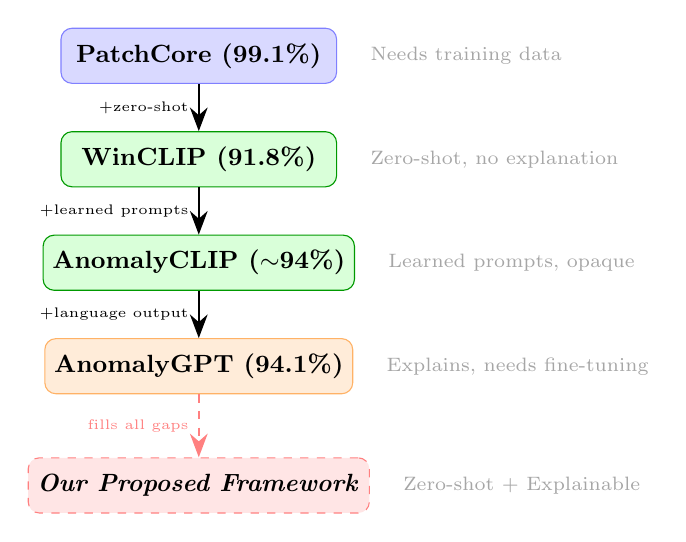
\begin{tikzpicture}[
    box/.style={rectangle, draw, rounded corners=4pt, minimum width=3.5cm, minimum height=0.7cm, text centered, font=\small\bfseries},
    arr/.style={-{Stealth[length=3mm]}, thick},
    note/.style={font=\scriptsize, text=gray!70}
]
% Nodes stacked vertically
\node[box, fill=blue!15, draw=blue!50] (pc) {PatchCore (99.1\%)};
\node[note, right=0.3cm of pc] {Needs training data};

\node[box, fill=green!15, draw=green!60!black, below=0.6cm of pc] (wc) {WinCLIP (91.8\%)};
\node[note, right=0.3cm of wc] {Zero-shot, no explanation};

\node[box, fill=green!15, draw=green!60!black, below=0.6cm of wc] (ac) {AnomalyCLIP ($\sim$94\%)};
\node[note, right=0.3cm of ac] {Learned prompts, opaque};

\node[box, fill=orange!15, draw=orange!60, below=0.6cm of ac] (ag) {AnomalyGPT (94.1\%)};
\node[note, right=0.3cm of ag] {Explains, needs fine-tuning};

\node[box, fill=red!10, draw=red!50, dashed, below=0.8cm of ag] (gap) {\textit{Our Proposed Framework}};
\node[note, right=0.3cm of gap] {Zero-shot + Explainable};

% Arrows
\draw[arr] (pc) -- node[left, font=\tiny] {+zero-shot} (wc);
\draw[arr] (wc) -- node[left, font=\tiny] {+learned prompts} (ac);
\draw[arr] (ac) -- node[left, font=\tiny] {+language output} (ag);
\draw[arr, dashed, red!50] (ag) -- node[left, font=\tiny] {fills all gaps} (gap);
\end{tikzpicture}
}%
\caption{Evolution of anomaly detection methods. Each step adds a capability (left labels) but introduces a new limitation (right annotations). Our proposed framework (dashed) targets the intersection of all desirable properties.}
\label{fig:evolution}
\end{figure}

\begin{table*}[t]
\centering
\caption{Comparative Overview of Surveyed Anomaly Detection Methods on MVTec AD}
\label{tab:comparison}
\renewcommand{\arraystretch}{1.4}
\begin{tabular}{|p{2.2cm}|p{1.3cm}|c|c|p{2.4cm}|c|p{1.8cm}|p{2.5cm}|}
\hline
\textbf{Method} & \textbf{Venue} & \textbf{Zero-Shot?} & \textbf{Img AUROC} & \textbf{Core Approach} & \textbf{Explains?} & \textbf{Training Needed} & \textbf{Chief Limitation} \\
\hline\hline
PatchCore~\cite{roth2022patchcore} & CVPR'22 & No & 99.1\% & Memory bank + KNN & No & Normal imgs per category & Not scalable to new domains \\
\hline
WinCLIP~\cite{jeong2023winclip} & CVPR'23 & Yes & 91.8\% & CLIP prompts + sliding window & No & None & Ad-hoc, hand-crafted prompts \\
\hline
AnomalyCLIP~\cite{zhou2024anomalyclip} & ICLR'24 & Yes$^*$ & $\sim$94\% & CLIP + learned prompts & No & Prompt optimisation & Requires training phase \\
\hline
AnomalyGPT~\cite{gu2024anomalygpt} & AAAI'24 & No & 94.1\% & Fine-tuned LVLM & Yes & Synthetic anomaly data & Fine-tuning required \\
\hline
MMAD~\cite{jiang2025mmad} & ICLR'25 & --- & --- & Benchmark / Evaluation & --- & --- & Evaluation framework only \\
\hline
\end{tabular}
\vspace{1mm}

\footnotesize{$^*$Zero-shot at test time, but requires a one-time prompt optimisation phase on labelled anomaly data.}
\end{table*}

Several patterns stand out from this comparison. First, there is a clear \textit{accuracy--flexibility trade-off}: PatchCore is the most accurate, but it is also the least flexible, because every new domain requires fresh training data. The CLIP-based methods sacrifice some accuracy in exchange for zero-shot generality. Second, there is a \textit{detection--explanation gap}: methods that detect well (PatchCore, WinCLIP, AnomalyCLIP) cannot explain their findings, while the one method that can explain (AnomalyGPT) cannot operate without task-specific fine-tuning. Third, the MMAD benchmark confirms that \textit{off-the-shelf MLLMs alone are insufficient}---even GPT-4o, the most capable commercial model tested, falls far short of dependable performance on anomaly-specific tasks.

These observations point toward a clear opportunity: a system that combines the reliable scoring of a CLIP-based VLM with the explanatory capacity of an open-source MLLM, without requiring any training or fine-tuning whatsoever.

% ============ 5. RESEARCH GAPS ============
\section{Identified Research Gaps}

Drawing on our analysis of the surveyed literature, we identify three specific gaps that the current body of work leaves unaddressed.

\textbf{Gap~1: No Principled Prompt Engineering Study for CLIP-Based Anomaly Detection.}\
WinCLIP selects its prompt templates and state words by hand, without any systematic investigation of why those particular choices work or how alternative designs might perform. AnomalyCLIP sidesteps the problem entirely by learning continuous prompts, but the learned vectors are opaque and the training requirement adds overhead. A middle ground---a structured, empirical study of how prompt template structure, state-word vocabulary, contextual phrasing, and ensemble composition each affect detection accuracy---is notably absent. Such a study would be valuable not only for anomaly detection but as a contribution to the broader prompt-engineering literature, since the principles are likely to generalise across visual grounding tasks.

\textbf{Gap~2: Limited Exploration of Open-Source MLLMs for Anomaly Reasoning.}\
AnomalyGPT convincingly demonstrates the value of combining an MLLM with anomaly detection, but its reliance on fine-tuning limits accessibility and scalability. The MMAD benchmark shows that off-the-shelf MLLMs (including proprietary ones) are not good enough on their own. What has not been explored is the potential of open-source MLLMs such as LLaVA \textit{when used in concert with a strong visual feature extractor like CLIP}. In this pairing, the MLLM would not need to independently detect the anomaly---it would only need to describe and reason about a region that CLIP has already flagged, a substantially easier task.

\textbf{Gap~3: No Hybrid VLM+MLLM Pipeline.}\
Every method we reviewed treats the VLM and the MLLM as separate, stand-alone tools. CLIP-based approaches (WinCLIP, AnomalyCLIP) perform scoring but offer no explanation. MLLM-based approaches (AnomalyGPT, raw MLLMs evaluated by MMAD) attempt both detection and explanation, but their detection accuracy is insufficient when used alone. A complementary, two-stage pipeline---first score with a VLM, then explain with an MLLM---has, to the best of our knowledge, not been investigated. Such a design would let each component operate in its zone of strength: CLIP handles the numerically demanding task of ranking regions by anomaly likelihood, while the MLLM applies its language-generation ability to produce human-readable reports.

% ============ 6. PROPOSED FRAMEWORK ============
\section{Proposed Research Direction}

Motivated by the gaps outlined above, we propose a two-stage hybrid framework for zero-shot, interpretable anomaly detection that is fully training-free and built on open-source components. Fig.~\ref{fig:pipeline} presents the overall architecture.

\begin{figure}[!ht]
\centering
\resizebox{0.85\columnwidth}{!}{%
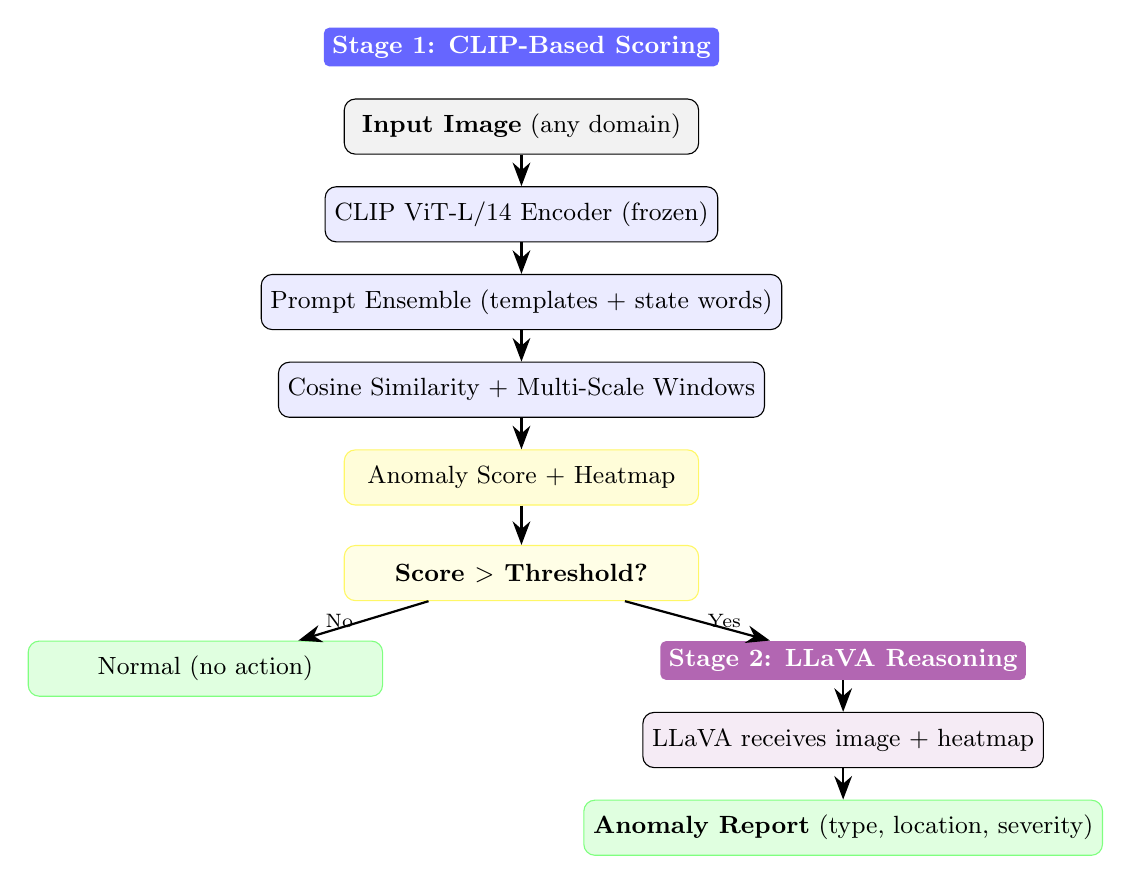
\begin{tikzpicture}[
    box/.style={rectangle, draw, rounded corners=4pt, minimum width=4.5cm, minimum height=0.7cm, text centered, font=\small},
    arr/.style={-{Stealth[length=3mm]}, thick},
    stglbl/.style={font=\small\bfseries, text=white, fill=blue!60, rounded corners=2pt, inner sep=3pt},
    stglbl2/.style={font=\small\bfseries, text=white, fill=violet!60, rounded corners=2pt, inner sep=3pt}
]

% Stage 1 label
\node[stglbl] (s1) {Stage 1: CLIP-Based Scoring};

% Stage 1 boxes
\node[box, fill=gray!10, below=0.4cm of s1] (input) {\textbf{Input Image} (any domain)};
\node[box, fill=blue!8, below=0.4cm of input] (clip) {CLIP ViT-L/14 Encoder (frozen)};
\node[box, fill=blue!8, below=0.4cm of clip] (prompt) {Prompt Ensemble (templates + state words)};
\node[box, fill=blue!8, below=0.4cm of prompt] (score) {Cosine Similarity + Multi-Scale Windows};
\node[box, fill=yellow!15, draw=yellow!60, below=0.4cm of score] (out1) {Anomaly Score + Heatmap};

% Decision
\node[box, fill=yellow!10, draw=yellow!60, below=0.5cm of out1] (dec) {\textbf{Score $>$ Threshold?}};

% No branch
\node[box, fill=green!12, draw=green!50, below left=0.5cm and -0.5cm of dec] (no) {Normal (no action)};

% Stage 2 label
\node[stglbl2, below right=0.5cm and -0.5cm of dec] (s2) {Stage 2: LLaVA Reasoning};

% Stage 2 boxes
\node[box, fill=violet!8, below=0.4cm of s2] (mllm) {LLaVA receives image + heatmap};
\node[box, fill=green!12, draw=green!50, below=0.4cm of mllm] (report) {\textbf{Anomaly Report} (type, location, severity)};

% Arrows
\draw[arr] (input) -- (clip);
\draw[arr] (clip) -- (prompt);
\draw[arr] (prompt) -- (score);
\draw[arr] (score) -- (out1);
\draw[arr] (out1) -- (dec);
\draw[arr] (dec) -- node[left, font=\scriptsize] {No} (no);
\draw[arr] (dec) -- node[right, font=\scriptsize] {Yes} (s2);
\draw[arr] (s2) -- (mllm);
\draw[arr] (mllm) -- (report);

\end{tikzpicture}
}%
\caption{Architecture of the proposed two-stage hybrid framework. Stage~1 uses CLIP for zero-shot scoring. Only flagged images proceed to Stage~2, where LLaVA generates a natural-language report.}
\label{fig:pipeline}
\end{figure}

\subsection{Research Question}

\textit{How can pre-trained Vision-Language Models and Multimodal Large Language Models be combined to perform zero-shot anomaly detection, achieving robust quantitative scoring alongside human-readable explanations, without any domain-specific training?}

\subsection{Stage~1: VLM-Based Anomaly Scoring}

The first stage uses a pre-trained CLIP model to compute anomaly scores at both image and pixel levels:
\begin{itemize}[leftmargin=*, itemsep=2pt]
    \item \textbf{Structured Prompt Engineering:}\ Rather than relying on ad-hoc prompt choices (WinCLIP) or learning opaque continuous prompts (AnomalyCLIP), we plan to carry out a systematic ablation across multiple dimensions of prompt design: template structure (declarative vs.\ interrogative vs.\ descriptive), state-word vocabulary (degree of specificity, positive vs.\ negative framing), contextual descriptions (with and without domain context), and ensemble composition (how many prompts, how they are combined). By conducting this study on a held-out set and evaluating on unseen categories, we aim to derive generalisable guidelines for prompt design in anomaly-related tasks.
    \item \textbf{Multi-Scale Windowed Features:}\ Following the approach established by WinCLIP, we apply overlapping sliding windows at multiple spatial resolutions to extract localised CLIP features. Each window's feature vector is compared against text prototypes via cosine similarity, and scores from all windows and scales are fused into a pixel-level anomaly heatmap.
    \item \textbf{Output:}\ An image-level anomaly score and a pixel-level heatmap identifying suspicious regions.
\end{itemize}

\subsection{Stage~2: MLLM-Based Reasoning and Explanation}

For images that Stage~1 flags as anomalous (i.e., whose score exceeds a calibrated threshold), the second stage invokes an open-source MLLM---currently LLaVA---to generate a natural-language report:
\begin{itemize}[leftmargin=*, itemsep=2pt]
    \item The MLLM receives the original image alongside the anomaly heatmap produced by Stage~1, together with a structured prompt that asks it to describe the flagged region, characterise the type of anomaly, estimate its extent, and comment on possible causes.
    \item Because the heavy-lifting of detection has already been done by CLIP, the MLLM does not need to independently identify the anomaly. It only needs to \textit{describe and reason about} a region that has already been highlighted, which plays to the strengths that current open-source MLLMs already possess.
    \item This design also keeps inference costs manageable: the computationally expensive MLLM is called only for the small fraction of images that cross the anomaly threshold, not for every single frame or sample in a data stream.
\end{itemize}

\subsection{Stage~3: Systematic Evaluation}

We plan to benchmark the proposed pipeline along two axes:
\begin{itemize}[leftmargin=*, itemsep=2pt]
    \item \textbf{Quantitative:}\ Image-level AUROC, pixel-level AUROC, and F1-score on MVTec~AD and VisA, compared against PatchCore, PaDiM (via the Anomalib library), WinCLIP, and AnomalyCLIP.
    \item \textbf{Qualitative:}\ Human evaluation of the MLLM-generated explanations for accuracy, relevance, and informativeness, drawing on the seven-subtask framework established by MMAD.
\end{itemize}

\subsection{Expected Contributions}

\begin{enumerate}[leftmargin=*, itemsep=3pt]
    \item A structured, empirical prompt-engineering study for CLIP-based anomaly detection, yielding reproducible guidelines for prompt design.
    \item A hybrid VLM+MLLM pipeline that pairs quantitative anomaly scores with natural-language explanations, with no fine-tuning required.
    \item A thorough benchmark comparing the proposed framework against both conventional and VLM-based baselines across multiple datasets.
    \item A demonstration of the framework's domain-agnosticism through application to visual domains beyond manufacturing, including potential extension to video-level anomaly detection (e.g., surveillance, medical imaging time series).
\end{enumerate}

\subsection{Novelty}

The novelty of this work rests on two pillars. First, the \textit{systematic prompt-engineering study} fills a gap that neither WinCLIP (which uses untested hand-crafted prompts) nor AnomalyCLIP (which avoids the question by learning prompts) has addressed. Second, the \textit{hybrid two-stage architecture} is, to our knowledge, the first approach to combine a VLM's scoring with an MLLM's reasoning in a single, training-free, open-source pipeline for anomaly detection.

% ============ 7. EXPERIMENTAL METHODOLOGY ============
\section{Experimental Methodology and Timeline}

\subsection{Experimental Setup}

Table~\ref{tab:setup} summarises the datasets, models, baselines, and metrics planned for the experimental phase.

\begin{table}[h]
\centering
\caption{Planned Experimental Resources}
\label{tab:setup}
\renewcommand{\arraystretch}{1.35}
\begin{tabular}{|p{1.8cm}|p{5.5cm}|}
\hline
\textbf{Component} & \textbf{Details} \\
\hline\hline
Datasets & MVTec AD (15 categories, 5,354 images); VisA (generalisation study) \\
\hline
VLM & OpenCLIP (ViT-B/32 and ViT-L/14) \\
\hline
MLLM & LLaVA (open-source, NeurIPS~2023) \\
\hline
Baselines & PatchCore, PaDiM (via Anomalib), WinCLIP, AnomalyCLIP \\
\hline
Metrics & Image-AUROC, Pixel-AUROC, F1-score; qualitative assessment of explanations \\
\hline
Frameworks & PyTorch, HuggingFace Transformers, Anomalib (Intel) \\
\hline
\end{tabular}
\end{table}


% ============ 8. CONCLUSION ============
\section{Conclusion}

This survey has examined the rapidly maturing landscape of multimodal anomaly detection. Conventional methods like PatchCore deliver near-perfect accuracy on established benchmarks but remain tethered to domain-specific training data and offer no insight into the anomalies they detect. CLIP-based zero-shot methods such as WinCLIP and AnomalyCLIP remove the training requirement and perform respectably, yet they cannot articulate what they have found. MLLM-based methods like AnomalyGPT bring conversational explanatory power to the table but sacrifice zero-shot generality by requiring fine-tuning. And the MMAD benchmark shows plainly that even the strongest commercial MLLMs are not yet ready to handle anomaly detection on their own.

The hybrid framework we propose---coupling CLIP's zero-shot scoring with LLaVA's open-source reasoning---targets the intersection of these capabilities. It aims for competitive detection accuracy, clear natural-language explanations, no domain-specific training, and full reproducibility through open-source components. By also conducting a principled prompt-engineering study, we hope to contribute not only a practical detection system but also a set of reusable insights into how textual prompts can be designed for visual anomaly grounding tasks across diverse application domains.

% ============ REFERENCES ============
\begin{thebibliography}{15}

\bibitem{bergmann2019mvtec}
P.~Bergmann, M.~Fauser, D.~Sattlegger, and C.~Steger,
``MVTec AD---A comprehensive real-world dataset for unsupervised anomaly detection,''
in \textit{Proc. IEEE/CVF Conf. Comput. Vis. Pattern Recognit. (CVPR)}, 2019, pp.~9592--9600.

\bibitem{radford2021clip}
A.~Radford, J.~W.~Kim, C.~Hallacy, A.~Ramesh, G.~Goh, S.~Agarwal, G.~Sastry, A.~Askell, P.~Mishkin, J.~Clark, G.~Krueger, and I.~Sutskever,
``Learning transferable visual models from natural language supervision,''
in \textit{Proc. Int. Conf. Mach. Learn. (ICML)}, 2021, pp.~8748--8763.

\bibitem{liu2023llava}
H.~Liu, C.~Li, Q.~Wu, and Y.~J.~Lee,
``Visual instruction tuning,''
in \textit{Proc. Adv. Neural Inf. Process. Syst. (NeurIPS)}, 2023.

\bibitem{roth2022patchcore}
K.~Roth, L.~Pemula, J.~Zepeda, B.~Sch{\"o}lkopf, T.~Brox, and P.~Gehler,
``Towards total recall in industrial anomaly detection,''
in \textit{Proc. IEEE/CVF Conf. Comput. Vis. Pattern Recognit. (CVPR)}, 2022, pp.~14318--14328.

\bibitem{jeong2023winclip}
J.~Jeong, Y.~Zou, T.~Kim, D.~Zhang, A.~Ravichandran, and O.~Dabeer,
``WinCLIP: Zero-/few-shot anomaly classification and segmentation,''
in \textit{Proc. IEEE/CVF Conf. Comput. Vis. Pattern Recognit. (CVPR)}, 2023, pp.~10175--10184.

\bibitem{zhou2024anomalyclip}
Q.~Zhou, G.~Pang, Y.~Tian, S.~He, and J.~Chen,
``AnomalyCLIP: Object-agnostic prompt learning for zero-shot anomaly detection,''
in \textit{Proc. Int. Conf. Learn. Represent. (ICLR)}, 2024.

\bibitem{gu2024anomalygpt}
Z.~Gu, B.~Zhu, G.~Zhu, Y.~Chen, M.~Tang, and J.~Wang,
``AnomalyGPT: Detecting industrial anomalies using large vision-language models,''
in \textit{Proc. AAAI Conf. Artif. Intell. (AAAI)}, 2024.

\bibitem{jiang2025mmad}
X.~Jiang, Y.~Cao, J.~Ge, and Z.~Lin,
``MMAD: A comprehensive benchmark for multimodal large language models in industrial anomaly detection,''
in \textit{Proc. Int. Conf. Learn. Represent. (ICLR)}, 2025.



\end{thebibliography}

\end{document}
